\let\negmedspace\undefined
\let\negthickspace\undefined
\documentclass[journal]{IEEEtran}
\usepackage[a5paper, margin=10mm, onecolumn]{geometry}
%\usepackage{lmodern} % Ensure lmodern is loaded for pdflatex
\usepackage{tfrupee} % Include tfrupee package

\setlength{\headheight}{1cm} % Set the height of the header box
\setlength{\headsep}{0mm}     % Set the distance between the header box and the top of the text

\usepackage{gvv-book}
\usepackage{gvv}
\usepackage{cite}
\usepackage{amsmath,amssymb,amsfonts,amsthm}
\usepackage{algorithmic}
\usepackage{graphicx}
\usepackage{textcomp}
\usepackage{xcolor}
\usepackage{txfonts}
\usepackage{listings}
\usepackage{enumitem}
\usepackage{mathtools}
\usepackage{gensymb}
\usepackage{comment}
\usepackage[breaklinks=true]{hyperref}
\usepackage{tkz-euclide} 
\usepackage{listings}
% \usepackage{gvv}                                        
\def\inputGnumericTable{}                                 
\usepackage[latin1]{inputenc}                                
\usepackage{color}                                            
\usepackage{array}                                            
\usepackage{longtable}                                       
\usepackage{calc}                                             
\usepackage{multirow}                                         
\usepackage{hhline}                                           
\usepackage{ifthen}                                           
\usepackage{lscape}
\begin{document}
\bibliographystyle{IEEEtran}
\vspace{3cm}

\title{6.2.6}
\author{EE25BTECH11060 - V.Namaswi}
% \maketitle
% \newpage
% \bigskip
{\let\newpage\relax\maketitle}
\renewcommand{\thefigure}{\theenumi}
\renewcommand{\thetable}{\theenumi}
\setlength{\intextsep}{10pt} % Space between text and floats
\textbf{Question}\\
Find matrix X such that\\
\begin{align*}
   X \begin{pmatrix}
        1 & 2 & 3\\
        4 & 5 & 6
    \end{pmatrix}= \begin{pmatrix}
        -7 & -8 & -9 \\ 2 & 4 & 6
    \end{pmatrix}
    \end{align*}\\
\textbf{Solution}\\
Form the augmented matrix  
\begin{align}
   \begin{pmatrix}
1 & 4 & | & -7 & -8 & -9 \\
2 & 5 & | & 2 & 4 & 6 \\
3 & 6 & | & 0 & 0 & 0
\end{pmatrix} \\ 
\end{align}
Replace $R_2 \to R_2-2R_1 $ and $R_3 \to R_3-3R_1$
\begin{align}
\begin{pmatrix}
1 & 4 & | & -7 & -8 & -9 \\
0 & -3 & | & 16 & 20 & 27 \\
0 & -6 & | & 21 & 24 & 27
\end{pmatrix} 
\end{align}
Replace $R_2 \to \frac{-1}{3}R_2$ and $R_3 \to R_3-2R_2$
\begin{align}
\begin{pmatrix}
1 & 4 & | & -7 & -8 & -9 \\
0 & 1 & | & -16/3 & -20/3 & -9 \\
0 & 0 & | & -11/3 & -16/3 & 9
\end{pmatrix}
\end{align}
Hence,
\begin{align}
    \Vec{X}=\begin{pmatrix}
    1 & 2\\
    -2 &  0
\end{pmatrix}
\end{align} 

 Pseudoinverse verification\\
Let,
\begin{align}
\Vec{A} = \begin{pmatrix}1 & 2 & 3 \\ 4 & 5 & 6\end{pmatrix}\\
\Vec{B} = \begin{pmatrix}-7 & 2 \\ -8 & 4 \\ -9 & 6\end{pmatrix} \\
\Vec{A}^+ &= \Vec{A}^\top (\Vec{A}\Vec{A}^\top)^{-1} \\  
= \begin{pmatrix}
-17/18 & 4/9 \\
-1/9 & 1/9 \\
13/18 & -2/9
\end{pmatrix} 
\end{align}
 \begin{align}
\Vec{X} &= \Vec{B}\Vec{A}^+ \\  
= \begin{pmatrix}-7 & 2 \\ -8 & 4 \\ -9 & 6\end{pmatrix} 
\begin{pmatrix}-17/18 & 4/9 \\ -1/9 & 1/9 \\ 13/18 & -2/9\end{pmatrix} \\ 
=\begin{pmatrix}1 & 2 \\ -2 & 0\end{pmatrix} 
\end{align}

    \centering
    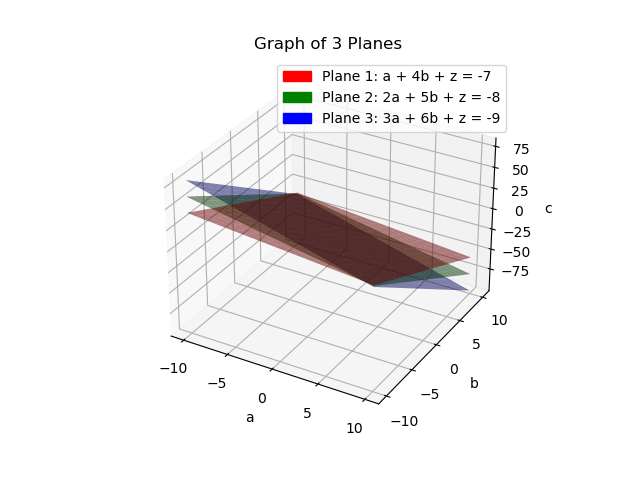
\includegraphics[width=\columnwidth, height=0.8\textheight, keepaspectratio]{figs/Figure_13.png}  
\end{document}
